%------------------------------%
%% ✎ Dylan (V1) %%%%%%%%% ✅ %%
%% ✎ Alain (V2) %%%%%%%%% ❌ %%
%% ✎ Dylan (V3) %%%%%%%%% ❌ %%
%------------------------------%

\afterpage{%
\afterpage{%

    % Arrière-plan partie III
    \AddToShipoutPictureBG*{%
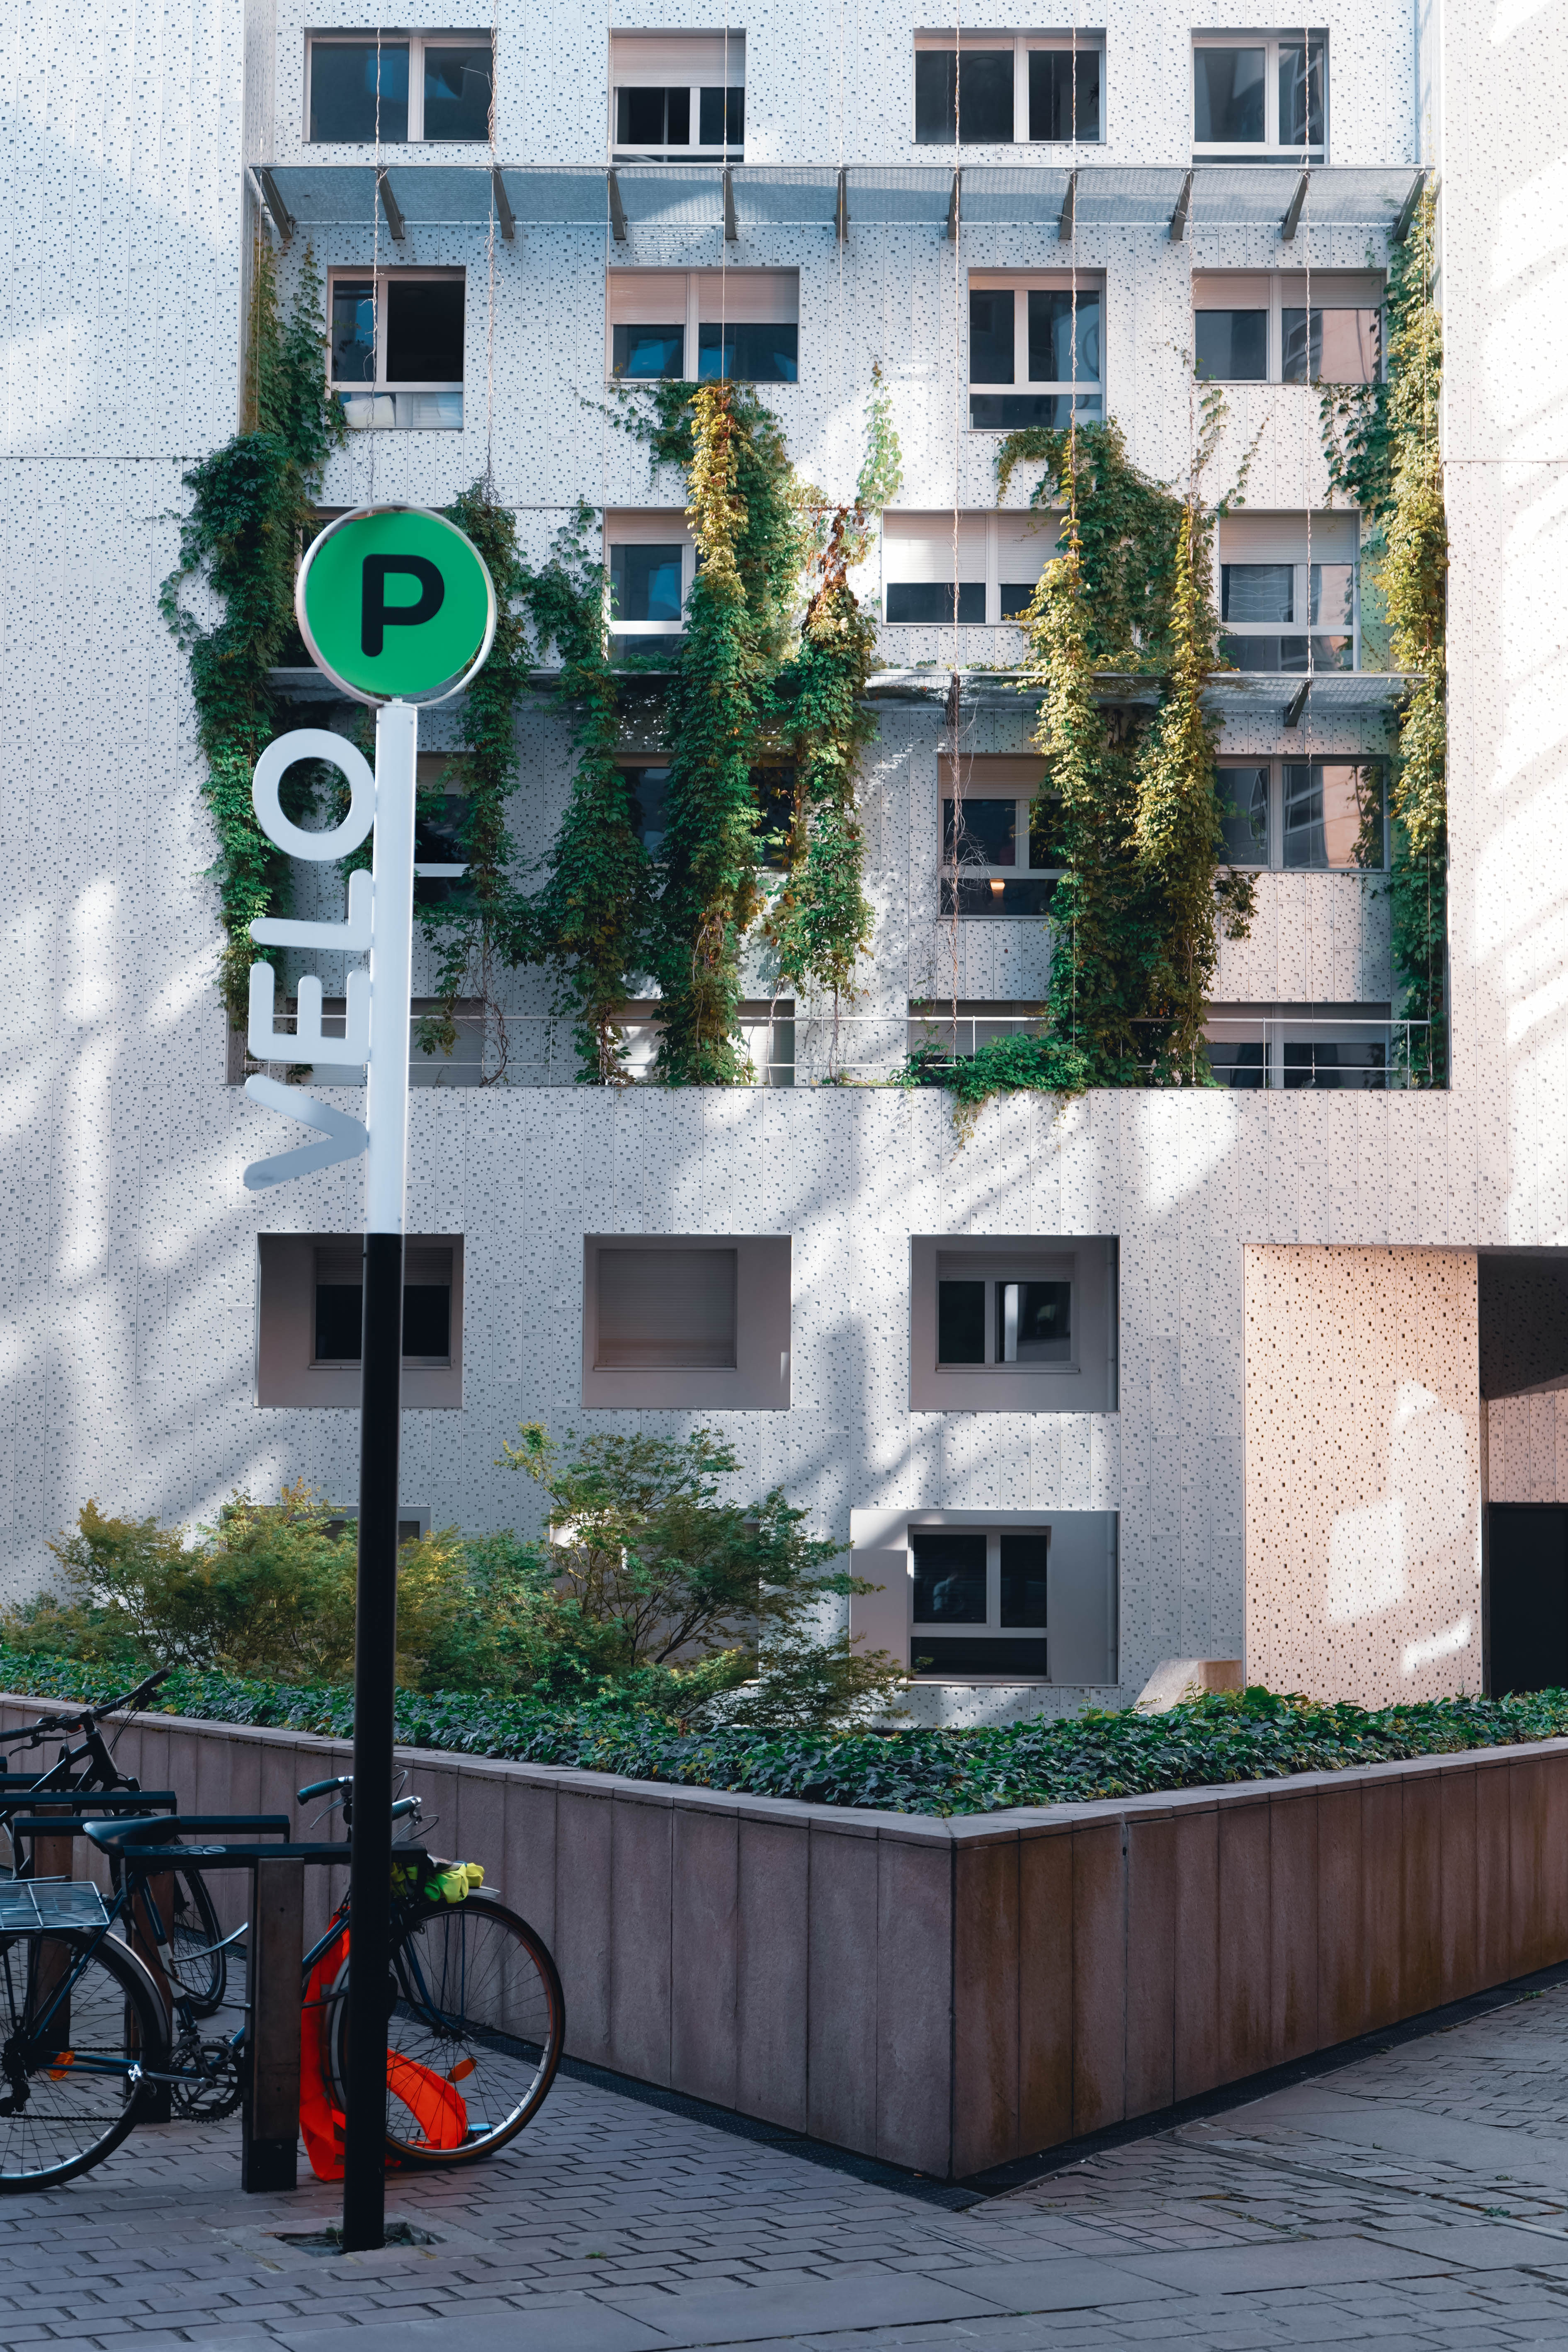
\includegraphics[width=\paperwidth,height=\paperheight]{src/Figures/Arriere_plan/Arriere_plan_Part_3.jpg}
    }

% Rectangle
\AddToShipoutPictureBG*{
  \begin{tikzpicture}[remember picture,overlay]
    \node[fill=white, opacity=0.75, text width=\paperwidth, minimum height=10cm, anchor=north] 
    at ([yshift=-7.7cm]current page.north) {};
  \end{tikzpicture}
}

% Source
\AddToShipoutPictureFG*{
  \AtPageLowerRight{
    \raisebox{1cm}{
      \hspace{16cm}
      
\begin{tikzpicture}
        \node[fill=white, rounded corners=5pt, inner sep=5pt, align=center] {
          \tiny{Photographie~: \textcolor{blue}{Dylan Moinse (2024)}}
        };
      \end{tikzpicture}
    }
  }
}
}}

\needspace{1\baselineskip} % Réserve de l'espace
\part{Formalisation pratique d'un système régional et intermodal, orienté vers le rail et soutenu par la mobilité individuelle légère
    \label{part3:titre}
    }
    \markboth{Partie~III~: Traduction fonctionnelle du \textsl{Micromobility-friendly Transit-Oriented Development}}{}
    \markright{Partie~III~: Traduction fonctionnelle du \textsl{Micromobility-friendly Transit-Oriented Development}}{}

% Introduction de la partie III
\cleardoublepage
\section*{Introduction de la partie~III
    \label{part3:introduction}
    }
    \addcontentsline{toc}{chapter}{Introduction de la partie~III}

    % Introduction
\lettrine[lines=3, findent=8pt, nindent=0pt]{\lettrinefont L}{es} analyses conceptuelles et empiriques développées dans les parties précédentes ont mis en évidence le rôle stratégique de la mobilité individuelle légère dans l’amélioration de l’accessibilité intermodale des quartiers de gare et son potentiel pour renouveler le modèle du \acrshort{TOD}. Elles ont montré que l’intégration de ces mobilités, bien que prometteuse, demeure encore fragmentaire et insuffisamment encadrée, tant sur le plan des infrastructures que des politiques publiques. Ces constats soulignent la nécessité de formaliser un cadre théorique et opérationnel structurant l’intégration de la mobilité individuelle au sein d'un \acrshort{M-TOD}, afin d’optimiser son efficacité et d’assurer une transition vers un urbanisme intermodal plus performant, résilient et inclusif. C’est dans cette perspective que cette troisième et dernière partie s’attache à proposer un modèle élargi du \acrshort{TOD}, que nous qualifions de \acrfull{M-TOD} et qui vise à repenser la structuration des territoires autour des réseaux de transport en commun à travers une approche intermodale mieux adaptée aux pratiques de mobilité qui se sont récemment déployées dans les territoires. Ces éléments convergent vers une même conclusion~: le \acrshort{TOD}, dans sa conception actuelle, ne prend pas encore en compte l’essor des nouvelles solutions de mobilité et doit évoluer pour mieux intégrer la mobilité individuelle légère comme un élément structurant de son fonctionnement. C’est à cette évolution que répond la formalisation du \acrshort{M-TOD}.

    % Chapitre 6
\textsl{Formalisation d'un Micromobility-friendly Transit-Oriented Development intégrant, de manière systémique, la mobilité individuelle légère dans les quartiers de gare} (\hyperref[objectif-6]{objectif~\(O_6\)}, page~\pageref{objectif-6}). \hyperref[chap6:titre]{Le sixième chapitre} (page~\pageref{chap6:titre}) met l'accent sur la formalisation de la déclinaison du concept d'aménagement, en la traduisant sous forme de stratégies urbaines. Il définit ainsi ses principes directeurs et identifie les conditions requises pour son bon déploiement dans les politiques d'aménagement et de transport. Cette formalisation repose sur une modélisation régionale, veillant à revisiter le modèle \Guillemets{nœud-lieu} en intégrant plusieurs dimensions~: les formes du réseau et les services du système ferroviaire~; le degré de développement urbain et la qualité de l'environnement bâti~; les connexions et la configuration des espaces publics au sein des quartiers de gare~; et la fréquentation temporelle des pôles d'échange. Une telle démarche, combinant les forces de la géographie et de la science des données, nous amène à identifier et à quantifier l'influence des différents facteurs sur l'attractivité du réseau de transport en commun. Elle nous conduit également à classer les gares et leurs environs, selon trois familles d'intervention à mettre en œuvre, en cohérence avec le \acrshort{TOD} à l'échelle piétonne, et avec le \acrshort{M-TOD} à l'échelle cyclable. Ce travail de modélisation est enrichi par une étude de cas portant sur un corridor ferroviaire, permettant de transposer les implications opérationnelles du modèle réinterprété. L’analyse de ces éléments aboutit à la proposition d'une feuille de route stratégique, articulant actions et recommandations pour inscrire durablement la mobilité individuelle légère dans la planification des transports et de l’aménagement urbain.%%Rédigé%%